\documentclass[10pt,xcolor=dvipsnames,compress]{beamer}

\usepackage{danny_theme}
\usepackage{danny_style}
\usepackage{hyperref}
%\usepackage[algoruled,longend]{algorithm2e}
\usepackage{array}
\usepackage{graphicx}
\usepackage{amsmath}
\newcolumntype{C}{>{\centering\arraybackslash} m{1.3in} }
\newcolumntype{M}{>{\centering\arraybackslash} m{1.in} }
\everymath{\displaystyle}
\long\def\/*#1*/{}

\beamertemplatenavigationsymbolsempty


%===============================================================================
% 					  Presentation Title and Author  
%===============================================================================
\title[Supercapacitor]{
Inadequecy Representation of Supercapacitor Batteries Models}
%\subtitle{Nonlinear Deformation in Metallic Materials}

\author[Danial Faghihi]{Danial Faghihi}

\institute[ICES]{Institute for Computational Engineering and Sciences (ICES)\\
$\quad~$The University of Texas at Austin
}

\date[\today]{\today}
%===============================================================================
%===============================================================================



\begin{document}

%===============================================================================
% SLIDE 00
%===============================================================================
\begin{frame}
\titlepage
\end{frame}

%===============================================================================
% SLIDE 00
%===============================================================================
\begin{frame}
\frametitle{Outline}
\vfill

\vspace{0.7in}
\tableofcontents
\vspace{0.7in}

\vfill
\end{frame}




%%%%%%%--------------------------------------------------------------------------------------------------------------------------
\section{Motivation}
%%%%%%%--------------------------------------------------------------------------------------------------------------------------
%===============================================================================
% SLIDE 00
%===============================================================================
\begin{frame}
\frametitle{Outline}
\vfill

\vspace{0.7in}
\tableofcontents[currentsection,currentsubsection] 
\vspace{0.7in}

\vfill
\end{frame}


%===============================================================================
% SLIDE 01
%===============================================================================
\begin{frame}
\frametitle{What are supercapacitors?}
\vfill


Supercapacitors are intermediate power/energy storage/supply devices that bridge the gap between \textit{electrolytic capacitors} and  \textit{rechargeable batteries}. They can provide
\begin{itemize}
\item higher energy density (capacitance) than capacitors
\item higher power density (faster charge delivery) than batteries
\item many more charge and discharge cycles than batteries
\end{itemize}

\begin{center}
\vspace{-0.06in}
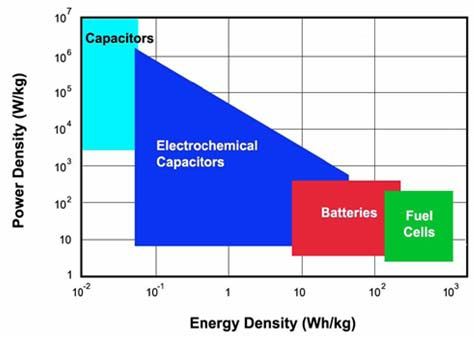
\includegraphics[trim = 0mm 0mm 0mm 0mm, clip, width=.48\textwidth]{figs/cap_battery}
\vspace{-0.1in}
\end{center}

\begin{small}
Supercapacitors are suitable in applications where a large amount of power is needed for a relatively
short time, where a very high number of charge/discharge cycles or a longer lifetime is required.
e.g. Low supply current for memory backup in SRAM, power for cars, etc.
\end{small}

\vfill
\end{frame}


%===============================================================================
% SLIDE 02
%===============================================================================
\begin{frame}
\frametitle{What are supercapacitors?}
\vfill


\begin{columns}[T] % contents are top vertically aligned
     \begin{column}[T]{6cm} % each column can also be its own environment
	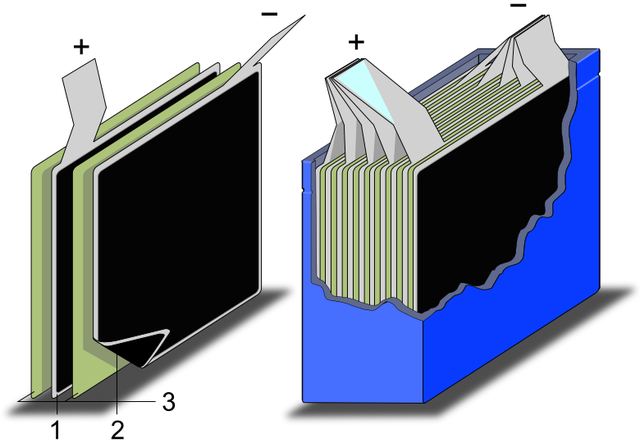
\includegraphics[trim = 0mm 0mm 0mm 0mm, clip, width=.7\textwidth]{figs/stacked.png}
	\\Supercapacitor with stacked electrodes
     \end{column}
     \begin{column}[T]{4cm} % alternative top-align that's better for graphics
	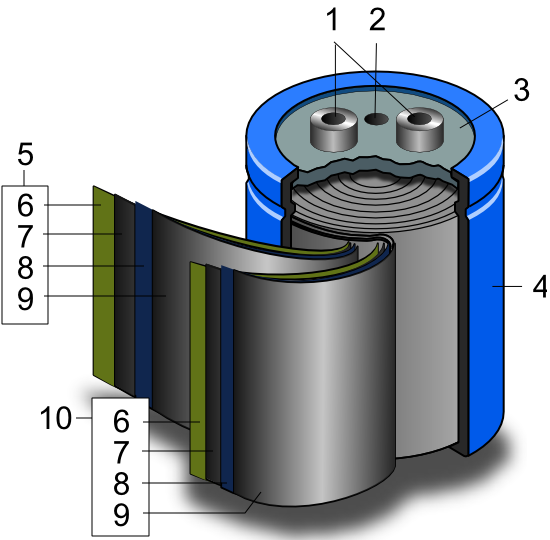
\includegraphics[trim = 0mm 0mm 0mm 0mm, clip, width=.7\textwidth]{figs/wound.png}
	\\ Wound supercapacitor
     \end{column}
\end{columns}

\begin{block}{}
\begin{columns}[T] % contents are top vertically aligned
     \begin{column}[T]{3cm} % each column can also be its own environment
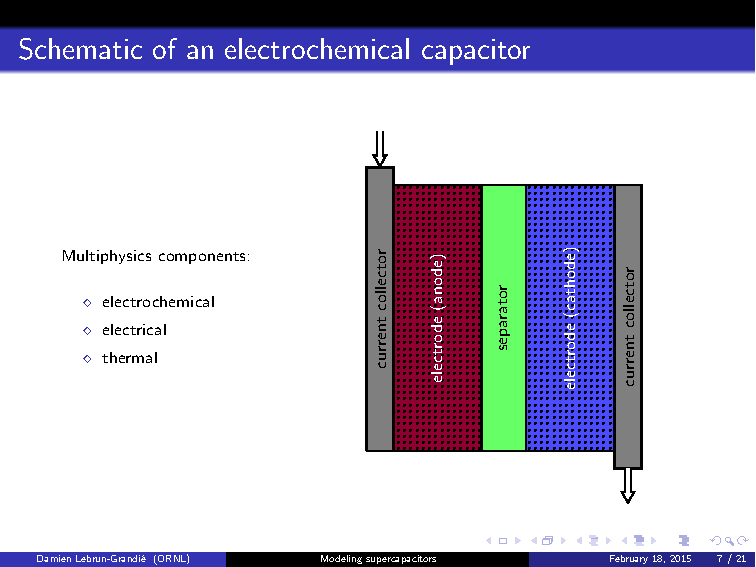
\includegraphics[trim = 2.4in 0.42in 0.7in 0.9in, clip, width=1\textwidth]{figs/supercap_schematic.pdf}  
    \end{column}
     \begin{column}[T]{7cm} % alternative top-align that's better for graphics
Unit cell:
\begin{itemize}
\begin{small}
\item Anode current collector
\item Porous anode electrode: solid matrix filled with liquid electrolyte
\item Separator: electronic insulator and ion permeable
\item Porous cathode electrode: solid matrix and liquid electrolyte
\item Cathode current collector.
\end{small}
\end{itemize}
     \end{column}
\end{columns}
\end{block}

\vfill
\end{frame}


%===============================================================================
% SLIDE 02
%===============================================================================
\begin{frame}
\frametitle{Storage principles}
\vfill

Capacitance value of an electrochemical capacitor is determined by two storage principles
\begin{itemize}
\item double-layer capacitance: electrostatic storage of the electrical energy
by separation of charge in a double layer at the interface between electrode/electrolyte .
The amount of electric charge stored is linearly proportional to the applied voltage and depends primarily on the electrode surface.
\item pseudo capacitance: electrochemical storage achieved by faradaic redox reactions with charge-transfer.
\end{itemize}

\begin{block}{}
explanations!!!
\end{block}


\vfill
\end{frame}


%%%%%%%--------------------------------------------------------------------------------------------------------------------------
\section{Model Description}
%%%%%%%--------------------------------------------------------------------------------------------------------------------------
%===============================================================================
% SLIDE 00
%===============================================================================
\begin{frame}
\frametitle{Outline}
\vfill

\vspace{0.7in}
\tableofcontents[currentsection,currentsubsection] 
\vspace{0.7in}

\vfill
\end{frame}


%===============================================================================
% SLIDE 03
%===============================================================================
\begin{frame}
\frametitle{Governing Equations}
\vfill

\begin{columns}
\begin{column}{.65\textwidth}
\begin{block}{electrode}
\textbf{Current density} following Ohm's law:
\begin{itemize}
\item Matrix phase :
$
i_1 = -\sigma\nabla\phi_1
$
\item Solution phase:
$
i_2 = -\kappa\nabla\phi_2
$
\end{itemize}
$\phi_1$, $\phi_2$: potentials,\\
$\sigma$, $\kappa$: electronic/ionic conductivity.
%

\vspace{0.1in}
\textbf{Conservation of charge:}
\vspace{-0.1in}
\begin{equation*}
-\nabla \cdot i_1 =  \nabla\cdot i_2 = a {i}_n
\vspace{-0.1in}
\end{equation*}
$a$: interfacial area per unit volume \\
${i}_n$: current transferred from the matrix to the electrolyte\\
$
{i}_n = \underbrace{C \frac{\partial}{\partial t} \eta}_{\rm double-layer} +
\underbrace{{i}_0 ( \exp (\frac{\alpha_aF}{RT}\eta) - \exp (-\frac{\alpha_aF}{RT}\eta)}_{\rm faradaic})
$

\vspace{0.1in}
overpotential: 
$
\eta =  \phi_1 - \phi_2.
$
\end{block}
\end{column}
%-----------------------------
\begin{column}{.30\textwidth} 
\begin{block}{collector}
\begin{equation*}
i_1 = -\sigma\nabla\phi_1
\end{equation*}
\begin{equation*}
-\nabla \cdot i_1 = 0
\end{equation*}
\end{block}
%%
\begin{block}{seperator}
\begin{equation*}
i_2 = -\kappa\nabla\phi_2
\end{equation*}
\begin{equation*}
-\nabla \cdot i_2 = 0
\end{equation*}
\end{block}
\end{column}
\end{columns}


\vfill
\end{frame}


%===============================================================================
% Slide 04
%===============================================================================
\begin{frame}
\frametitle{High Fidelity Model}
\vfill

\begin{columns}
\begin{column}{.47\textwidth}
\begin{itemize}
\begin{small}
\item $\eta(\xi,\tau)$ = overpotential in electrode\\
\item $\gamma = \frac{\kappa}{\sigma}$ : conductivity ratio \\
\item $\xi, \tau$ : dimensionless distance/time \\
\item $I(\tau)$ : dimensionless current
\end{small}
\end{itemize}
\end{column}
%-----------------------------
\begin{column}{.47\textwidth} 
	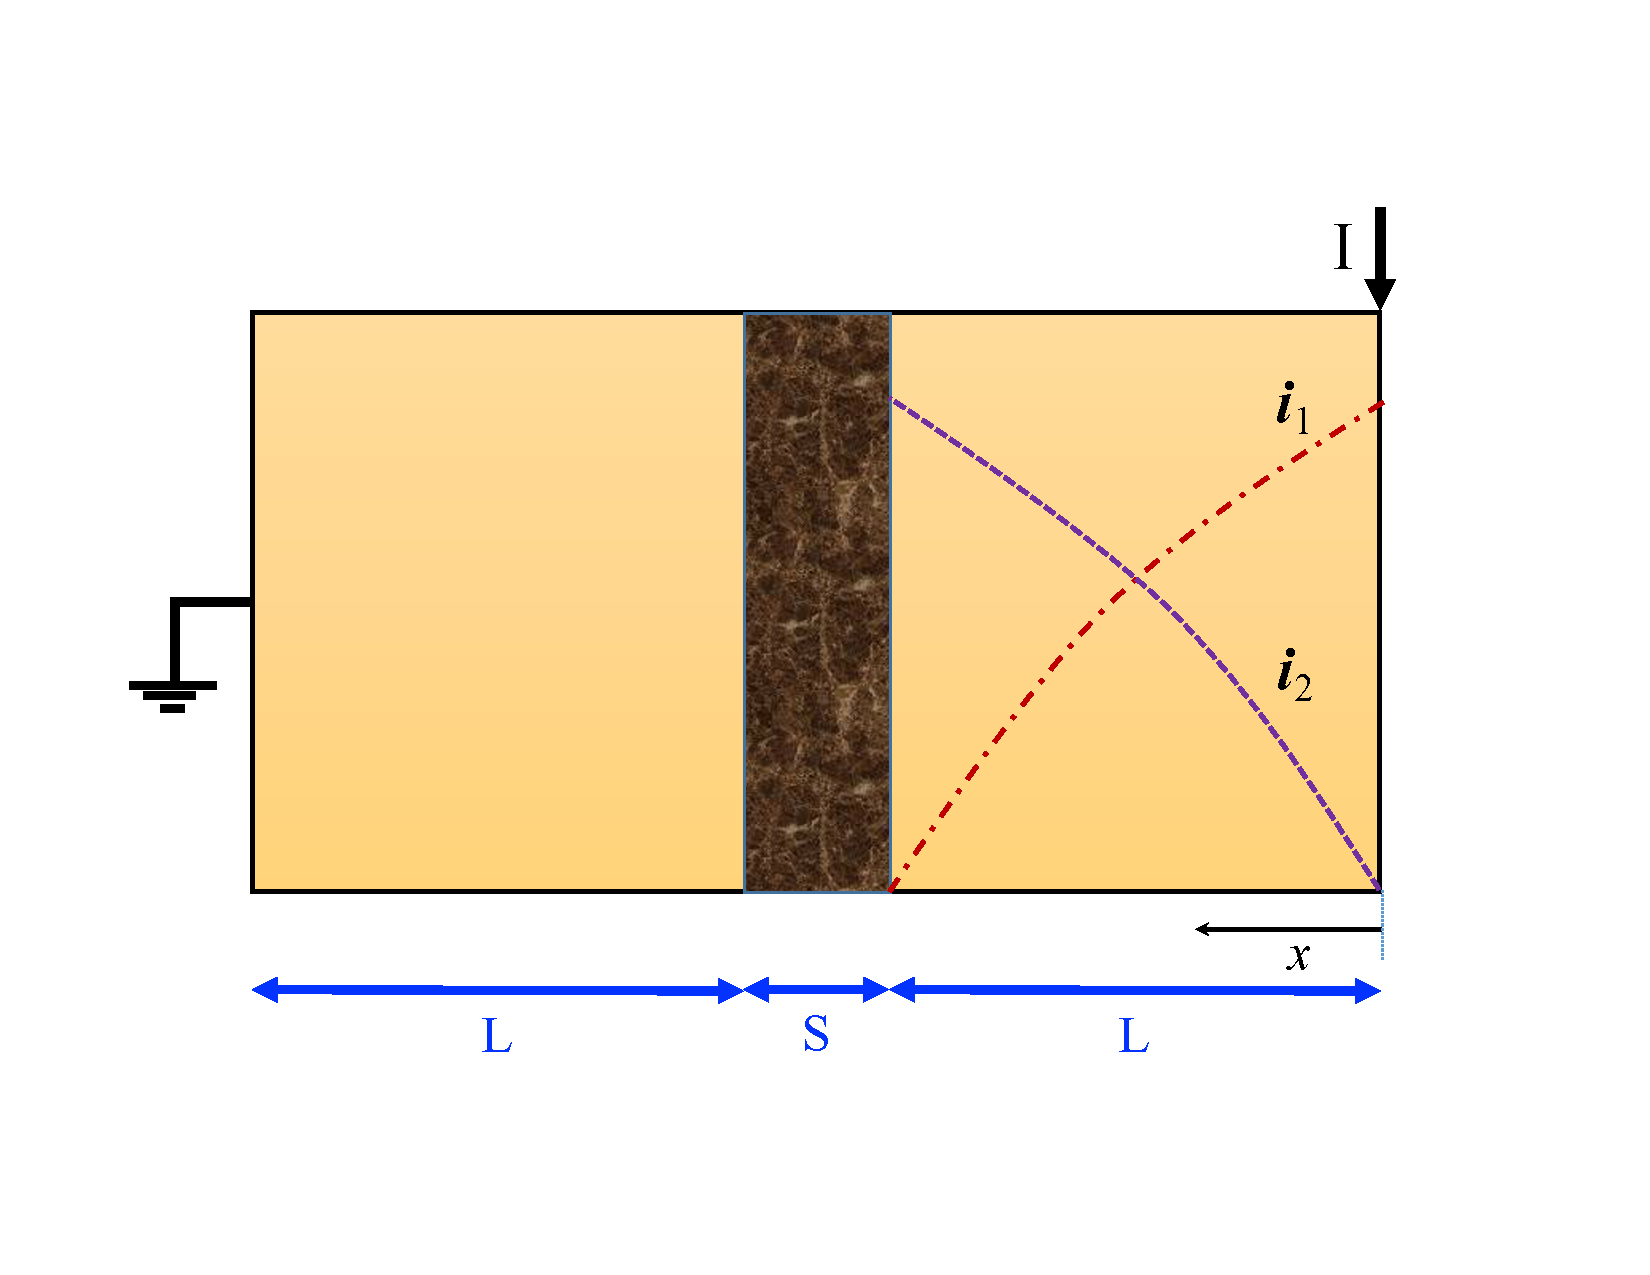
\includegraphics[trim = 0in 1.4in 0in 1.4in, clip, width=1\textwidth]{figs/schematic.pdf}
\end{column}
\end{columns}
%%====================
\begin{columns}
\begin{column}{.47\textwidth}
%-----------------------------
\begin{problock}{High Fidelity (1D) model}
\begin{equation*}\label{eq:HF}
\frac{\partial\eta}{\partial\tau} = \frac{\partial^2\eta}{\partial\xi^2}
\end{equation*}
\begin{equation*}
\left\{\begin{matrix}
\frac{\partial\eta}{\partial\xi}|_{\xi=0} & = & -\frac{\gamma}{1+\gamma}I(\tau)\\
\frac{\partial\eta}{\partial\xi}|_{\xi=1} & = & \frac{1}{1+\gamma}I(\tau) \nonumber\\
\eta|_{\tau=0} 					       & =  & \eta_0(\xi)
\end{matrix}\right.
\end{equation*}
\end{problock}
\end{column}
%-----------------------------
\begin{column}{.47\textwidth}
\vspace{-0.1in}
\begin{alertblock}{Modeling Assumptions (Sins)}
\begin{enumerate}[i.]

\begin{footnotesize}
\item No Faradaic processes:
current transferred from matrix to the solution phase goes towards only charging the double-layer at the electrode/electrolyte interface.

\item $\phi_1$ is uniformly distributed over the current collector domain (collector is sufficiently thin)
%
%The electrical resistivity of the current collector is low (or it is sufficiently thin) that one can assume uniform distribution of $\phi_1$ over the collector domain: \textit{homogeneous in the $x$-direction}, 

\item There is no electron/ion fluxes cross the top and bottom boundaries
%. Also due to high conductivity of collectors, the voltage over the whole interface on the collector side is negligible (similar to case that tab on the left collector is grounded): \textit{2D domain could be reduced to a quasi-1D domain},

\item The material properties are constant within each layer
\end{footnotesize}

\end{enumerate}
\end{alertblock}
\end{column}
\end{columns}


\vfill
\end{frame}


%===============================================================================
% Slide 05
%===============================================================================
\begin{frame}
\frametitle{Low Fidelity Model}
\vfill


\begin{alertblock}{Modeling Assumptions (Sins)}
\begin{enumerate}[i.]

\item Spatially
averaging the governing equation over the entire domain length (PDE of the HF model reduces to an ODE) 
%
\begin{equation}\label{eq:LF_avg}
\eta^{avg} = \int_0^1 \eta d\xi \qquad \Rightarrow \qquad
\frac{\partial{\eta}^{avg}}{\partial\tau} = I^*
\end{equation}

\item Assuming a quadratically varying profile for overpotential inside the electrodes
\begin{equation*}\label{eq:quadratic}
\eta_{LF} (\xi,\tau)= a(\tau)\xi^2 + b(\tau)\xi + c(\tau)
\end{equation*}
where $a$, $b$, and $c$ can be obtained from PDE+BCs of HF model.

\end{enumerate}
\end{alertblock}

%-----------------------------
\begin{block}{Low Fidelity (0D) model}
\begin{equation*}\label{eq:LF}
\eta_{LF}(\xi,\tau) = 
\frac{1}{2}I^*(\tau)\xi^2 - I^*(\tau) \frac{\gamma}{1+\gamma}\xi + {\eta}^{avg}(\tau) - \frac{I^*(\tau)}{6} + \frac{I^*(\tau)}{2}\frac{\gamma}{1+\gamma}
\end{equation*}
${\eta}^{avg}$ is the solution of (\ref{eq:LF_avg}) given appropriate initial condition.
\end{block}


\vfill
\end{frame}



%===============================================================================
% Slide 06
%===============================================================================
\begin{frame}
\frametitle{QoI : cell voltage }
\vfill


\begin{columns}
\begin{column}{.47\textwidth}
%-----------------------------
\begin{alertblock}{Quantity of Interest}
 Potential drop across the system
 \begin{eqnarray*}
 V^{\rm cell}(\tau) &=& \phi_{\rm col.}^L - \phi_{\rm col.}^R \\
 		&=& 2V_0 - 2V^{\rm elect.} - V^{\rm sep.}
 \end{eqnarray*}

where 

$
V^{\rm elect.}(\tau) =  \frac{1+2\gamma}{1+\gamma}\eta|_{\xi=1} - \frac{\gamma}{1+\gamma}\eta|_{\xi=0} 
 - \frac{\gamma}{(1+\gamma)^2}I
$
\end{alertblock}

\end{column}
%--------------------------------------
\begin{column}{.53\textwidth}
\begin{center}
%\vspace{-4mm}
\begin{figure}[h]
    \centering
    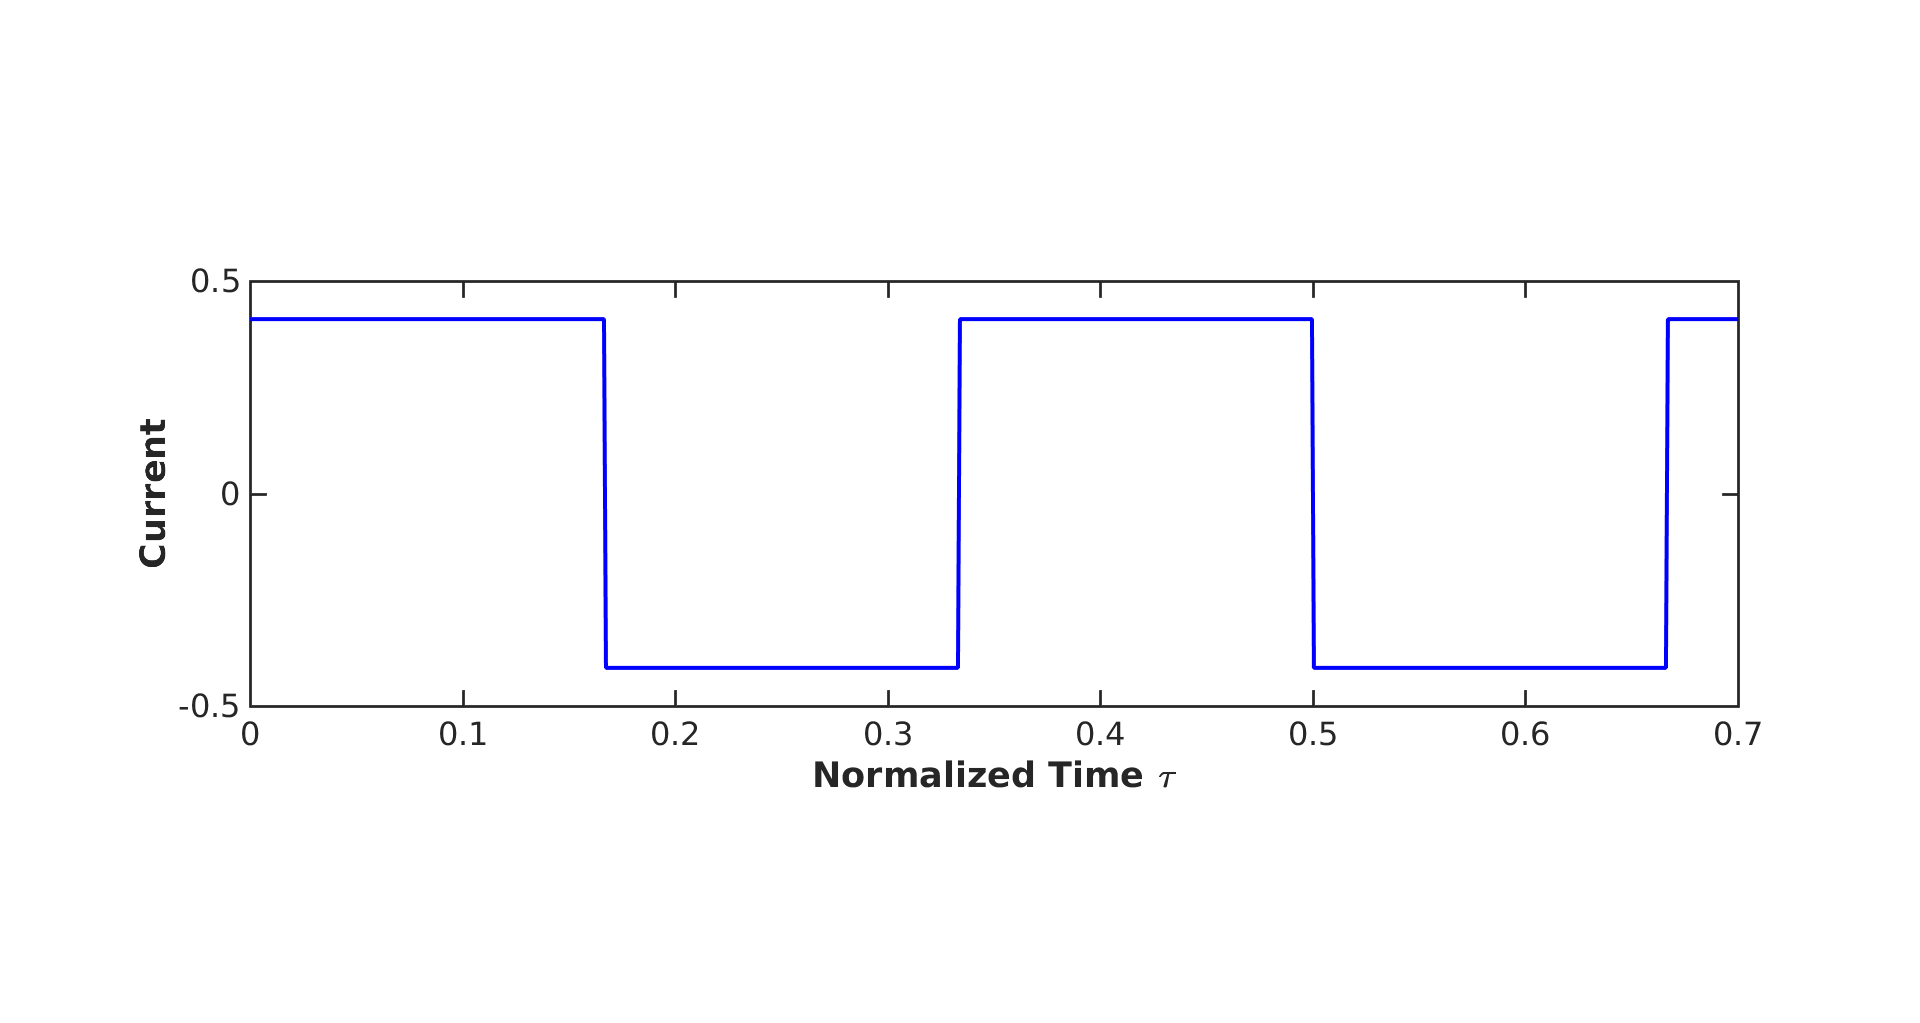
\includegraphics[trim = 1.2in 2.4in 1.6in 2.8in, clip, width=1\textwidth]{figs/I.png}
    \\
    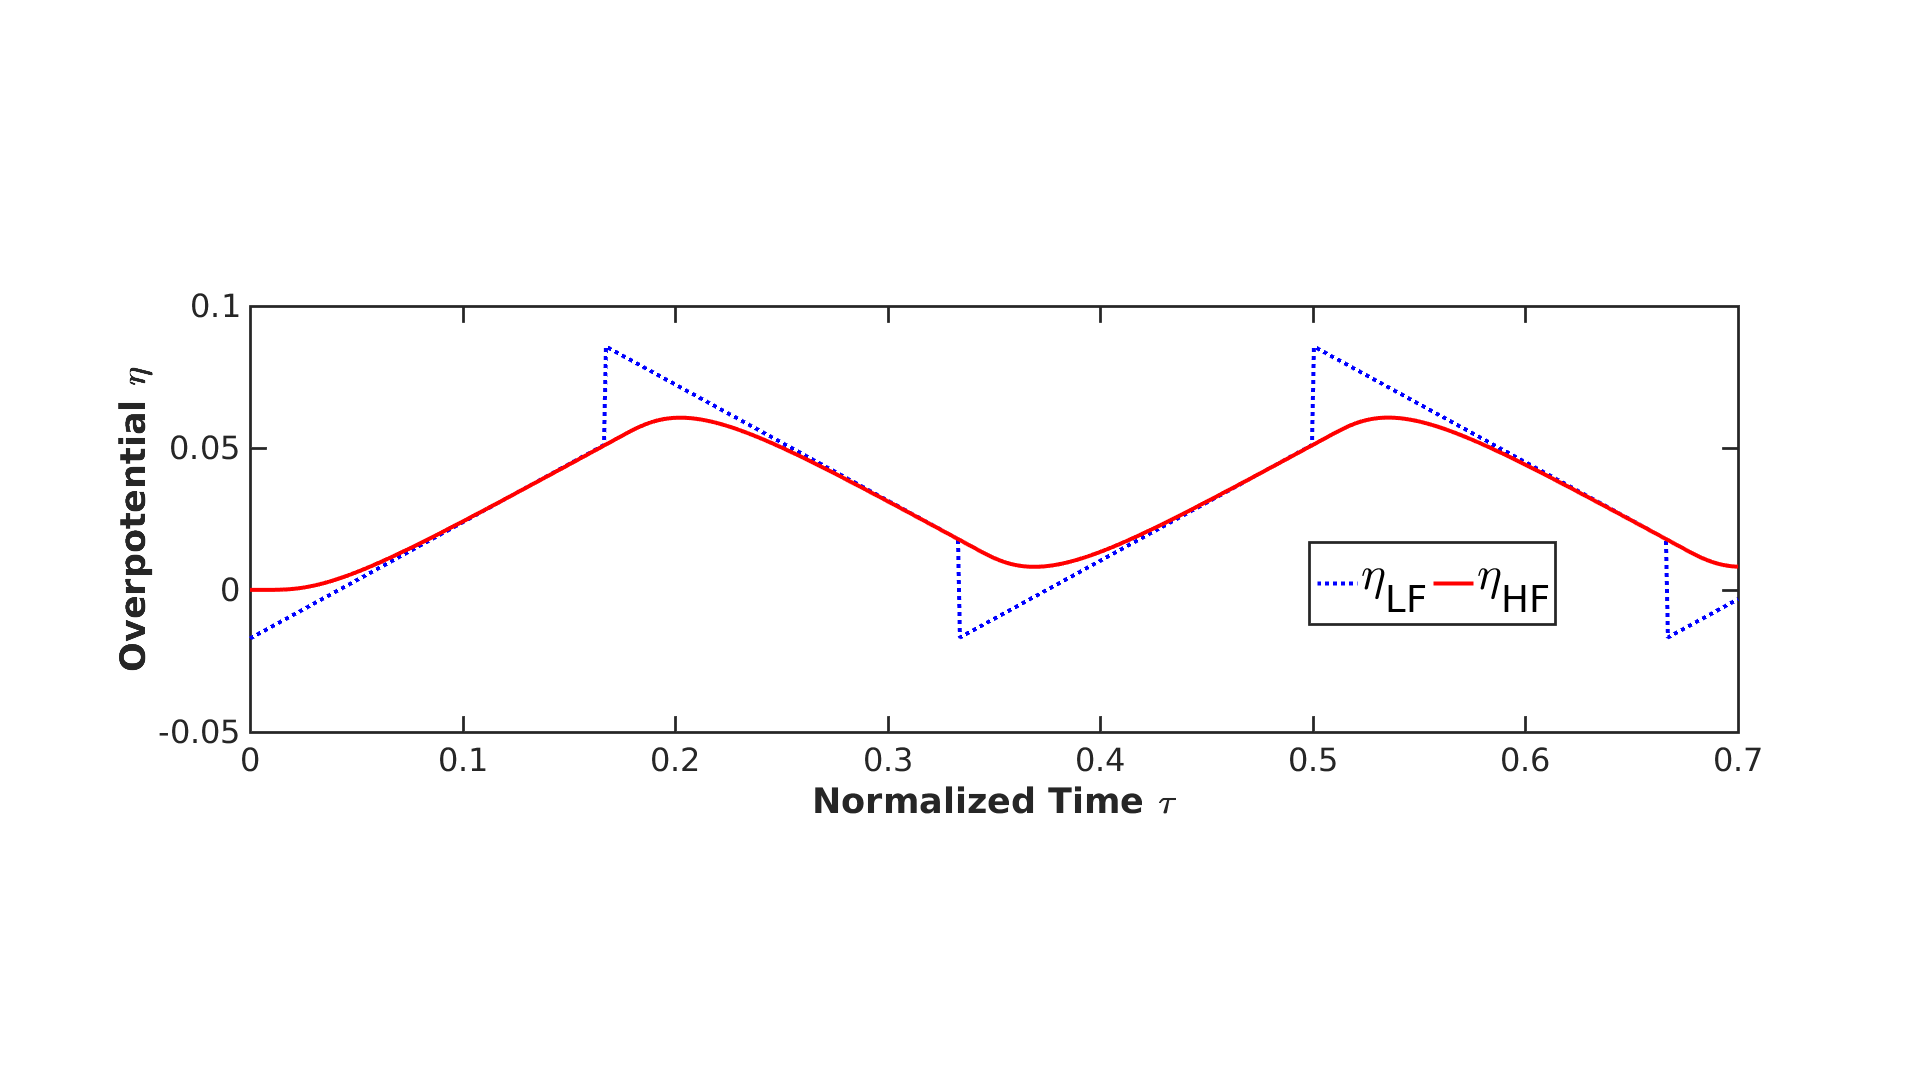
\includegraphics[trim = 1.2in 2.4in 1.6in 2.8in, clip, width=1\textwidth]{figs/etaLF_HF.png}   
    \\
    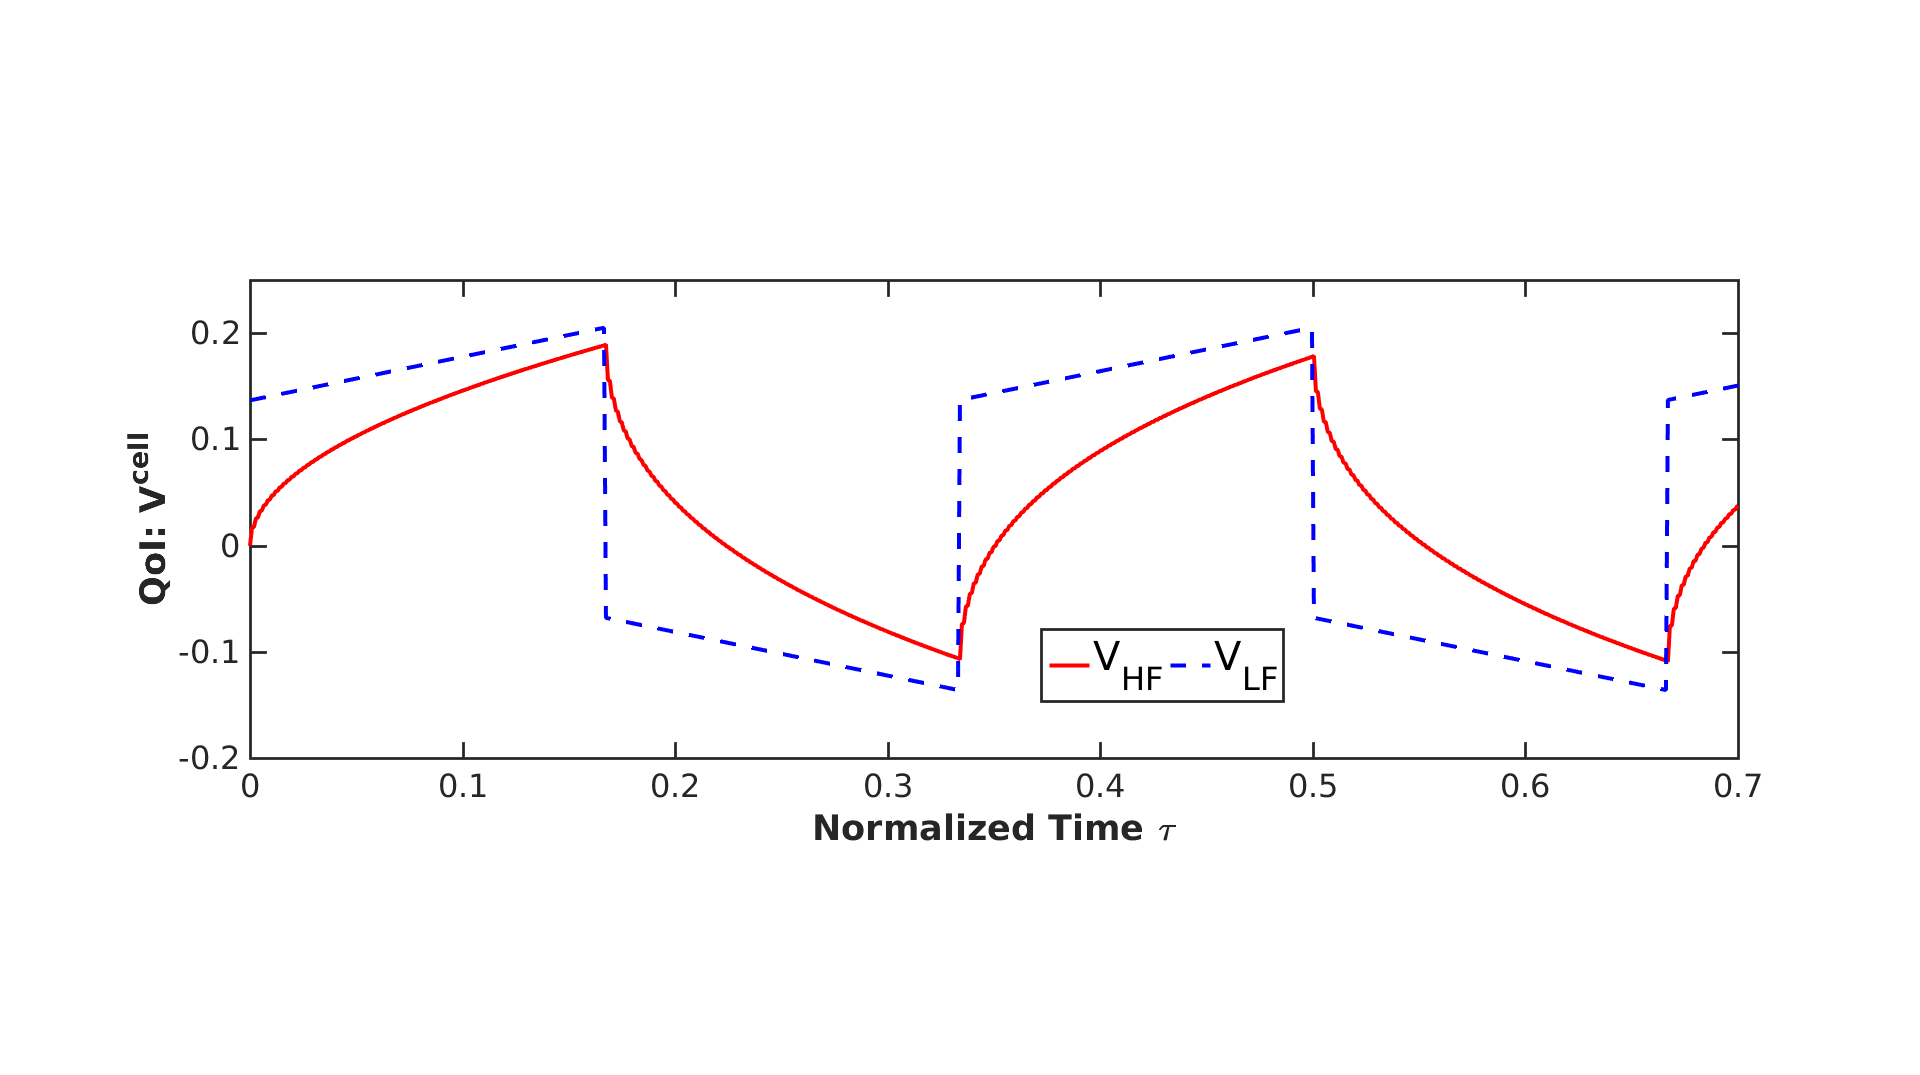
\includegraphics[trim = 1.2in 2.4in 1.6in 2.8in, clip, width=1\textwidth]{figs/Vcell_HF_LF.png} 
\end{figure}
\end{center}
\end{column}
\end{columns}


\vfill
\end{frame}



%%%%%%%--------------------------------------------------------------------------------------------------------------------------
\section{Inadequecy Representation}
%%%%%%%--------------------------------------------------------------------------------------------------------------------------
%===============================================================================
% SLIDE 00
%===============================================================================
\begin{frame}
\frametitle{Outline}
\vfill

\vspace{0.7in}
\tableofcontents[currentsection,currentsubsection] 
\vspace{0.7in}

\vfill
\end{frame}

%===============================================================================
% Slide 07
%===============================================================================
\begin{frame}
\frametitle{Model Inadequacy}
\vfill

We are interested in Error in QoI: \quad $\epsilon = V^{\rm cell}_{\rm HF} - V^{\rm cell}_{\rm LF}  \equiv V^{\rm electrode}_{\rm HF} - V^{\rm electrode}_{\rm LF} $\\
Given what we know about high fidelity model $\eta_{HF}$, we can formulate inadequacy representation. 

\begin{problock}{}
\begin{itemize}
\item Solution of low fidelity model converges to high fidelity over time i.e. modeling error is larger for higher frequency current. 
\item The high fidelity model accounts for the time history of the current. Such history does not appear with right dependency in the low fidelity model: 
%
\begin{small}
\begin{eqnarray*}
V^{\rm electrode}_{\rm HF} =& A(\gamma)\int_0^{\tau} I(\tau') \mathcal{K}(\tau-\tau') d\tau' &+ B(\gamma) I(\tau)\\
V^{\rm electrode}_{\rm LF} =& C(\gamma)\int_0^{\tau} I(\tau') d\tau' &+ D(\gamma) I(\tau)
\end{eqnarray*}
Solving PDE using Laplace transform
\[
\textstyle{
\mathcal{K}(\tau-\tau') = 
 \sum_{n=1}^\infty  e^{-n^2\pi^2(\tau-\tau')}d\tau'
}
\]
\end{small}
\item The stochastic inadequacy representation needs to account for the incomplete and uncertain history information available to the LF model.
\end{itemize}
\end{problock}


\vfill
\end{frame}


%===============================================================================
% Slide 08
%===============================================================================
\begin{frame}
\frametitle{Model Inadequacy}
\vfill


\begin{columns}
\begin{column}{.42\textwidth}
%-----------------------------
\begin{alertblock}{Inadequacy representation}
\textbf{Auxiliary Stochastic ODE:}
\begin{equation*}
\frac{\partial\epsilon}{\partial\tau} = -\lambda\epsilon + \alpha \frac{\partial I}{\partial\tau}
\end{equation*}

where $\lambda$ is a stochastic process with following time evolution:
\begin{equation*}
\frac{\partial\lambda}{\partial\tau} = -c(\lambda - \lambda_{mean}) + \beta \frac{\partial W}{\partial\tau}
\end{equation*}

where $W(\tau)$ is a Wiener process.% and $(\alpha, \beta, c, \lambda_{mean})$ are parameters of inadequacy representation. 
\end{alertblock}

\end{column}
%--------------------------------------
\begin{column}{.59\textwidth}
\begin{center}
%\vspace{-4mm}
\begin{figure}[h]
    \centering
    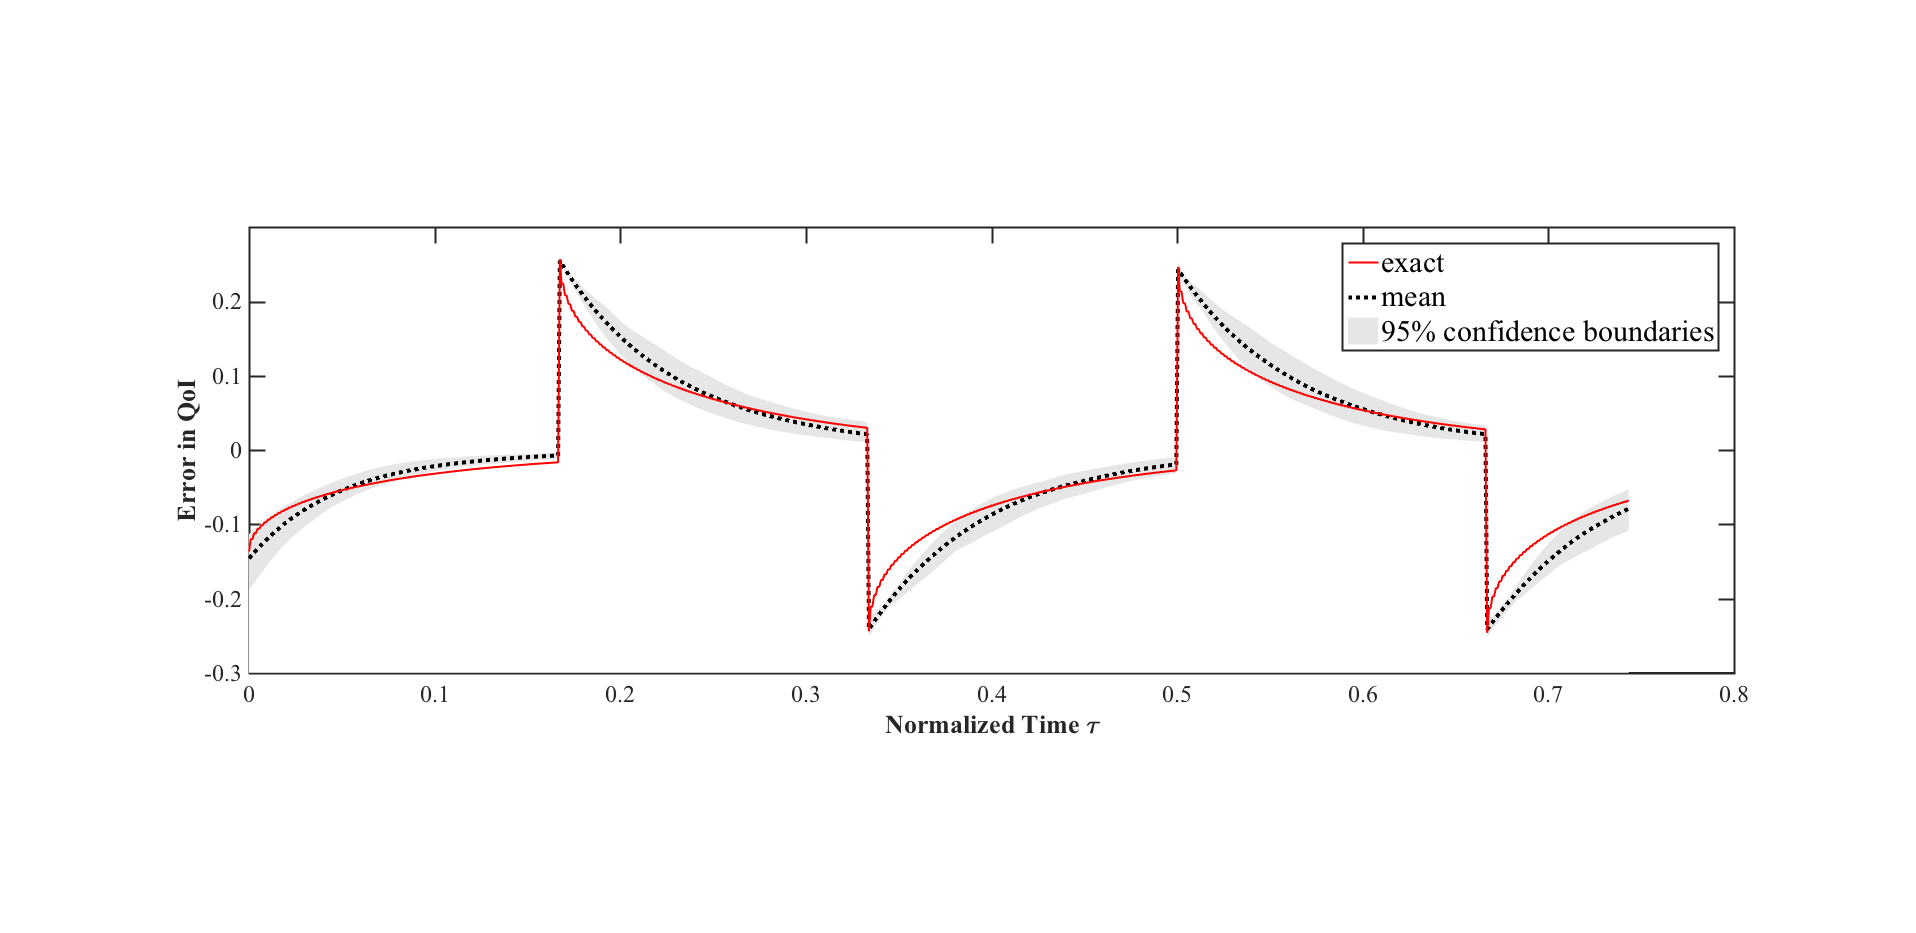
\includegraphics[trim = 1.3in 2.2in 1.6in 2.8in, clip, width=1\textwidth]{figs/error_bound.png} 
        \\
    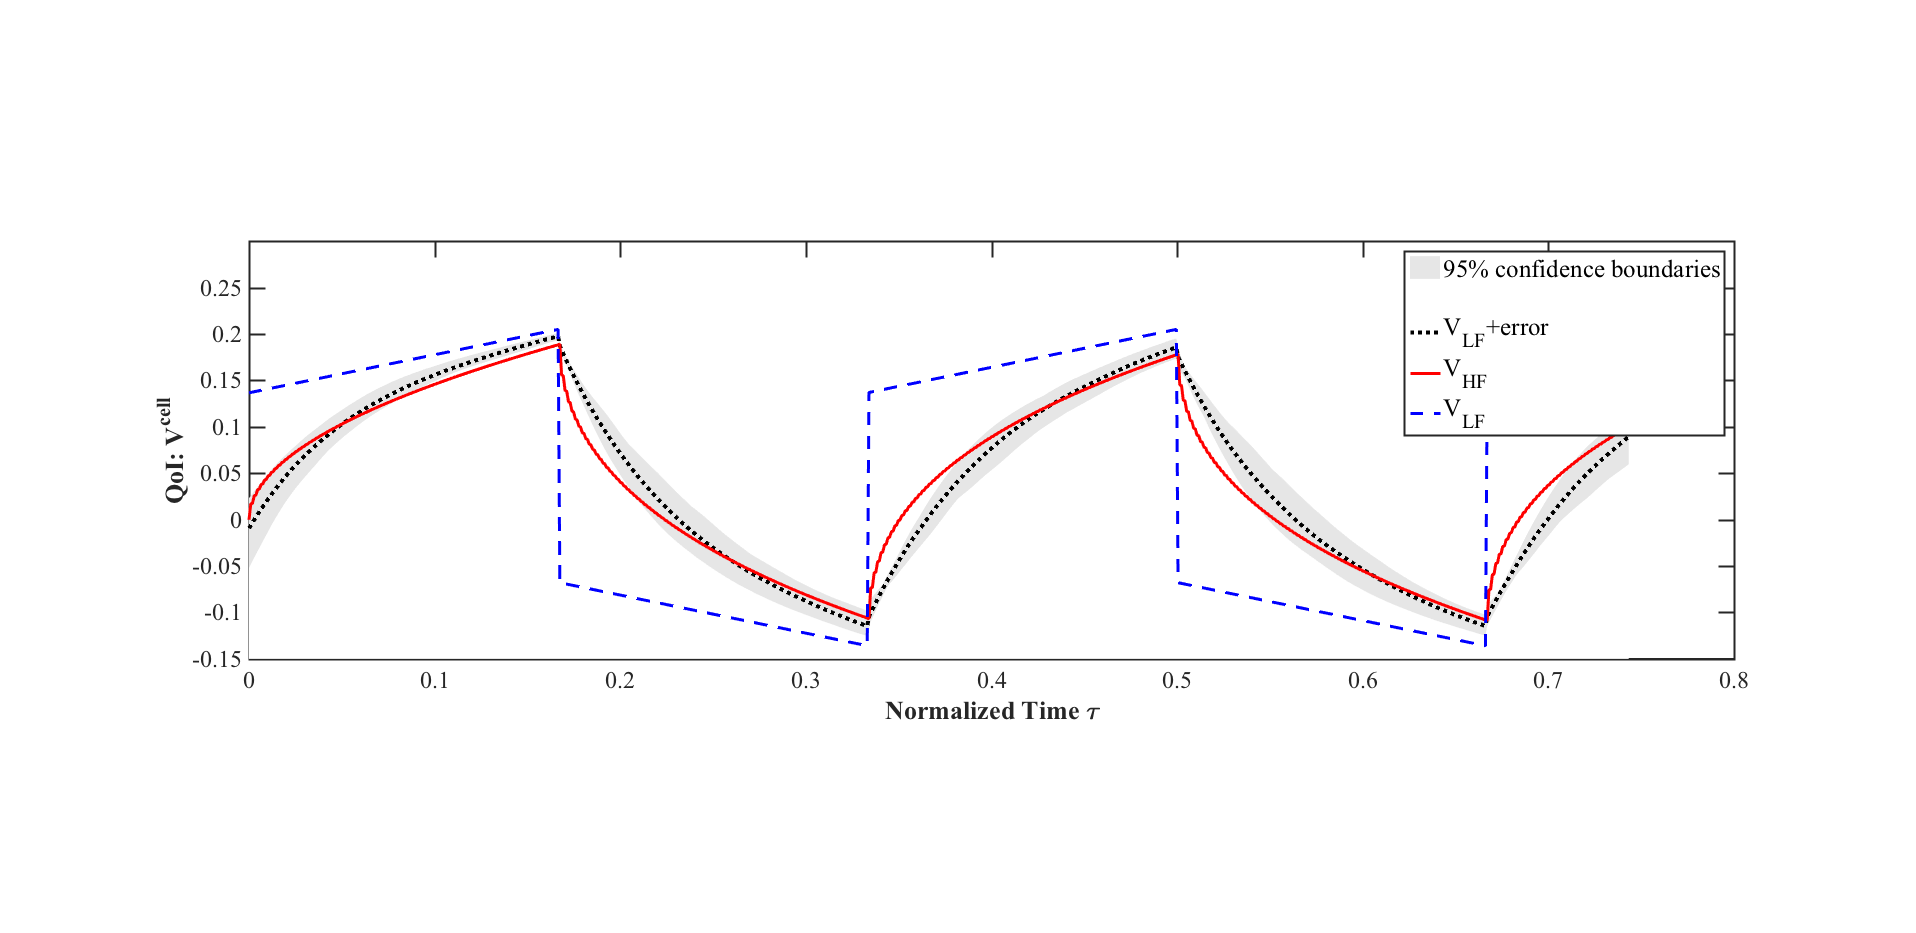
\includegraphics[trim = 1.3in 2.2in 1.6in 2.8in, clip, width=1\textwidth]{figs/V_bound.png} 
\end{figure}
\end{center}
\end{column}
\end{columns}
%====================
\begin{block}{}
\begin{itemize}
\item The ODE accounts for some of hidden features of HF i.e. $\lambda\epsilon$ takes care of the Kernel $\mathcal{K}$.
\item It needs to be trained by HF data.
\end{itemize}
\end{block}


\vfill
\end{frame}



\end{document}
